\documentclass[12pt,a4paper]{article}

\usepackage{amsmath,amssymb,amsfonts,amsthm}
\usepackage{mathtools}
\usepackage{fullpage,setspace}
\usepackage{caption}
\usepackage{subcaption}
\usepackage{enumitem}
\usepackage{float}
\usepackage{framed}
\usepackage{fancyhdr}
\usepackage[colorinlistoftodos]{todonotes}
\usepackage[english]{babel}
\usepackage[utf8]{inputenc}
\usepackage{algorithm}
\usepackage{algpseudocode}
\usepackage{verbatim}
\usepackage{algorithmicx}
\usepackage{mathrsfs}
\usepackage{booktabs}
\usepackage{titling}
%\usepackage{array}
\usepackage{multicol}
\usepackage{float}
\usepackage{graphicx}
\graphicspath{images}
\usepackage{indentfirst} % indent first paragraph
\usepackage{hyperref} % table of content links
\hypersetup{
    colorlinks=true,
    allcolors=black
}
\usepackage[top=.5in, bottom=1in, left=.5in, right=.5in]{geometry}
%\newcommand{\addpic}[1]{\includegraphics[width=14em]{#1}}
%\newcolumntype{C}{>{\centering\arraybackslash}m{14em}}

\title{APMA 1360: Homework Assignment \#1}
\pretitle{\begin{center}\fontsize{20bp}{18bp}\selectfont}
\posttitle{\par\end{center}}
\author{Eli Berkowitz}
\predate{}
\date{Feb 8 2017}
\postdate{}

\begin{document}

\maketitle

\section{Question 1}

Let $f(u) = \dot{u}$.
\begin{enumerate}[label = (\roman*)]
    \item Every real number is an equilibrium.
    $$f(u) = 0$$
    \item Every integer is an equilibrium, and there are no other fixed points besides those.
    $$f(u) = \sin{\pi u}$$
    \item There are exactly two equilibria and both are stable.

    This is impossible (proof).
    \item There are no equilibria.
        $$f(u) = u^2 + 1$$
    \item The flow looks like this:
    \begin{figure}[H]
        \centering
        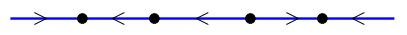
\includegraphics[width=0.7\textwidth]{flow-chart}
    \end{figure}
    A solution could be a polynomial such as:
    $$f(u) = -(u - 1) (u - 2)^{2} (u - 3)(u - 4)$$
    \begin{figure}[H]
        \centering
        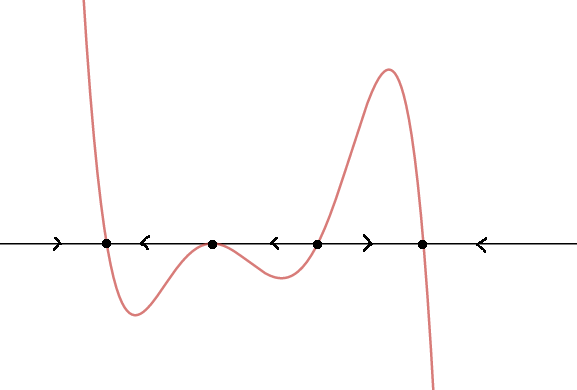
\includegraphics[width=0.7\textwidth]{flow-chart-soln}
    \end{figure}

    \item The flow has a periodic orbit $u(t)$
    $$f(u) = \sin{u}$$
\end{enumerate}
\section{Question 2}
Let:
$$\dot{u} = ru\left(1 - \frac{u}{K}\right) - \mu u$$

\begin{enumerate}[label = (\roman*)]
    \item
        \begin{itemize}
            \item Equilibria
            \begin{align}
            \dot{u} = 0 \implies ru\left(1 - \frac{u}{K}\right) - \mu u = 0 \\
            \implies u = \{0, \frac{k(r - \mu)}{r}\}
            \end{align}
            \item Stability

            Near $u_1 = 0$ (ignoring negative solutions since they're meaningless in this application), $f'(u_1) = r - \mu$. In other words, if the reproduction rate is greater than the harvest rate, the population grows. Otherwise, it shrinks to zero.

            On the other hand, near  $u_2 = \frac{k(r - \mu)}{r}$, $f'(u_2) = \mu - r$. Therefore, when the harvest rate is greater than the reproduction rate, $f'$ is positive so this equilibrium is unstable and the fish population will decline to zero (assuming no change in $\mu$). Otherwise, $f'(u_2) < 0 \implies$ the equilibrium is stable, so $u$ approaches this value.
        \end{itemize}
    \item Bifurcation Diagram

    Assuming $\mu > r$:

    \begin{figure}[H]
        \centering
        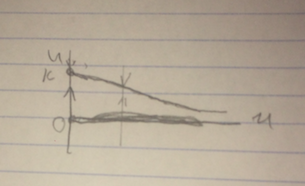
\includegraphics[width=0.7\textwidth]{bifurcation-diagram}
    \end{figure}

    \item The carrying capacity is the maximum sustainable population of fish when there is no harvesting (plugging in $\mu = 0$ in $f(u)$). A non-zero population will approach $k$ over time provided that harvesting greater than the reproduction rate does not start.

    The main idea to take away from this analysis is that fish harvesting will not result in the decline of a fish population unless it occurs faster than the reproduction of those fish (which makes complete sense!).

\end{enumerate}


\section{Question 3}

\begin{enumerate}[label = (\roman*)]
\item This paper at the very least attempts to appeal to broad audiences. Much of the language is broad, and there are no equations which are sure to intimidate those lacking a sound mathematical background. Large diagrams and logical yet surprisingly complex and detailed examples give the reader a way to grasp the mathematics in connection to the real world. Large diagrams give a powerful tool for visualization, making the authors' points much clearer to understand without a complete understanding of topology or catastrophe theory.

\item The paper largely does a good job at appealing to a generally broad audience. However, this is not the kind of paper you would be likely to share with a non-sciency friend. Complex terminology is rapidly introduced (sometimes relying on the reader learning the definitions from figure captions). At times the example is obscured by the attention being paid to the terminology, and it becomes difficult to keep track of both catastrophe theory and dog aggression models.

A remedy for this type of problem would be to use simpler jargon (which is certainly possible but with the consequence of somewhat reducing the learning of the reader), or introducing a little more mathematics so as not to lull the reader into the sense that the paper will be an easy read (which happened to me the first time through). The paper is in no way simple, but with an extravagant introduction and illustrations of dogs throughout the first few pages, it is difficult to take it completely seriously in the beginning.

As another note, I find long, small font captions difficult to parse, but that may just be personal.

\item Having large illustrations and simple examples that can be easily understood initially but have lots of hidden depth is a powerful mechanism to helping your audience understand your topic. Sometimes, one equation tells all the words of one figure, but having the figure increases the audience span tenfold, and that is often worth the extra ink.

\end{enumerate}

\section{Question 4}

If $f(u) = \dot{u}$, the equilibria of $f$ are the values $u_i$ such that $f(u_i) = 0$. Interpreted physically, equilibra are the points where the velocity or time rate of change of a position are zero and therefore will not change more unless the system is in some way changed or perturbed.

An equilibria is stable when even small perturbations in the system will not change the state of the solution. Mathematically speaking, this occurs when $f'(u_i) < 0$. This is because when $f'(u_i) < 0$, $f$ is positive close to the left of $u_i$, meaning the solution moves rightwards towards the equilibrium. Righward of the point, $f$ is negative, meaning the solution moves leftwards towards the solution. Either way, the particle will end up at $u_i$ and small perturbations will result in its return to $u_i$.


\end{document}
